\documentclass{ximera}

\author{Anna Davis \and Paul Zachlin} \title{Image and Kernel of a Linear Transformation} \license{CC-BY 4.0}

\renewcommand{\vec}[1]{{\bf #1}}
\newcommand{\RR}{\mathbb{R}}
\newcommand{\dfn}{\textit}
\newcommand{\dotp}{\cdot}

\newtheorem{general}{Generalization}
\newtheorem{initprob}{Exploration Problem}
\usepackage{tikz-cd}
\usetikzlibrary{shapes.geometric}
\usetikzlibrary{arrows}
\pgfplotsset{compat=1.14}



\begin{document}
\begin{abstract}
  We define the image and kernel of a linear transformation and prove the Rank-Nullity Theorem for linear transformations.
\end{abstract}
\maketitle

%Note to Student:  In this module we will often use $V$ and $W$ to denote the domain and codomain of linear transformations.  If you are familiar with abstract vector spaces, you can regard $V$ and $W$ as finite-dimensional vector spaces, otherwise you may think of $V$ and $W$ as subspaces of $\RR^n$. 

\section*{The Image of a Linear Transformation}
\begin{definition}\label{def:imageofT}
Let $V$ and $W$ be vector spaces, and let $T:V\rightarrow W$ be a linear transformation.  The image of $T$, denoted by $\text{im}(T)$, is the set
$$\text{im}(T)=\{T(\vec{v}):\vec{v}\in V\}$$
In other words, the image of $T$ consists of individual images of all vectors of $V$.
\end{definition}

\begin{example}\label{ex:image1}
Consider the linear transformation $T:\RR^3\rightarrow \RR^2$ with standard matrix
$$A=\begin{bmatrix}1&2&3\\2&4&6\end{bmatrix}$$

\begin{enumerate}
\item\label{item:impart1}
Find $\text{im}(T)$.
\item\label{item:impart2}
Illustrate the action of $T$ with a sketch.

\end{enumerate}
\begin{explanation}

\ref{item:impart1} Let $\vec{v}=\begin{bmatrix}a\\b\\c\end{bmatrix}$ then

$$T(\vec{v})=A\vec{v}=\begin{bmatrix}1&2&3\\2&4&6\end{bmatrix}\begin{bmatrix}a\\b\\c\end{bmatrix}=a\begin{bmatrix}1\\2\end{bmatrix}+b\begin{bmatrix}2\\4\end{bmatrix}+c\begin{bmatrix}3\\6\end{bmatrix}$$

Thus, every element of the image can be written as a linear combination of the columns of $A$.  We conclude that 
$$\text{im}(T)=\text{span}\left(\begin{bmatrix}1\\2\end{bmatrix}, \begin{bmatrix}2\\4\end{bmatrix}, \begin{bmatrix}3\\6\end{bmatrix}\right)=\text{col}(A)$$

Every column of $A$ is a multiple of $\begin{bmatrix}1\\2\end{bmatrix}$.  So, the image of $T$ is a line in $\RR^2$ determined by the vector $\begin{bmatrix}1\\2\end{bmatrix}$.

\ref{item:impart2} The action of $T$ can be illustrated with a sketch.

\begin{image}
\centering
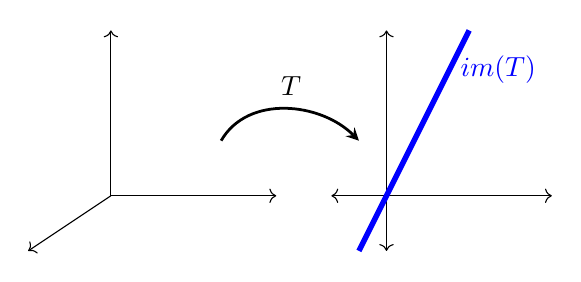
\begin{tikzpicture}[scale=.7]

  \draw[->] (0,0)--(3,0);
  \draw[->] (0,0)--(0,3);
  \draw[->] (0,0)--(-1.5,-1);

  
  \draw[<->] (4,0)--(8,0);
  \draw[<->] (5,-1)--(5,3);
  \draw[line width=2pt,blue](4.5,-1)--(6.5,3) node[below=5mm, left=-10mm]{$\text{im}(T)$};
  
  \draw [->,line width=1pt,-stealth]  (2,1) to[out=60] (4.5, 1)node[above=7mm, left=6mm]{$T$};
 % to[out=-20,in=-70] original command

\end{tikzpicture}
%\caption{The domain and the image of $T$.}
  \label{fig:actionofst} 
\end{image}


\end{explanation}
\end{example}

\begin{general}
In Example \ref{ex:image1} we observed that the image of the linear transformation was equal to the column space of its standard matrix.  In general, it is easy to see that if $T:\RR^n\rightarrow \RR^m$ is a linear transformation with standard matrix $A$ then
$$\text{im}(T)=\text{col}(A)$$


% Recall that the span of any collection of vectors of $\RR^m$ is a subspace of $\RR^m$ {\color{red} insert reference}.  Thus, $\text{im}(T)$ is a subspace of $\RR^m$. This justifies the following definition.

% \begin{definition}\label{def:rankofTRn}
% The rank of a linear transformation $T:\RR^n\rightarrow \RR^m$, is the dimension of the image of $T$.
% $$\text{rank}(T)=\text{dim}(\text{im}(T))$$
% \end{definition}


\end{general}
\begin{example}\label{ex:image2}
Let $T:\RR^5\rightarrow \RR^4$ be a linear transformation with standard matrix $$A=\begin{bmatrix}1 & 2 & 2 &-1 & 0\\-1 & 3 & 1 & 0 & -1\\3 & 0 & 0 & 3 & 6\\ 1 & -1 & 1 & -2 & -1\end{bmatrix}$$
Find $\text{im}(T)$ and $\text{dim}(\text{im}(T))$.
\begin{explanation}
As in Example \ref{ex:image1}, we find that the image of $T$ is given by
$$\text{im}(T)=\text{span}\left(\begin{bmatrix}1\\-1\\3\\1\end{bmatrix}, \begin{bmatrix}2\\3\\0\\-1\end{bmatrix}, \begin{bmatrix}2\\1\\0\\1\end{bmatrix}, \begin{bmatrix}-1\\0\\3\\-2\end{bmatrix}, \begin{bmatrix}0\\-1\\6\\-1\end{bmatrix}\right)=\text{col}(A)$$
But this time, it is harder to detect redundant vectors in the spanning set.  We have to rely on the reduced row-echelon form of $A$.

$$\begin{bmatrix}1 & 2 & 2 &-1 & 0\\-1 & 3 & 1 & 0 & -1\\3 & 0 & 0 & 3 & 6\\ 1 & -1 & 1 & -2 & -1\end{bmatrix}  \rightsquigarrow \begin{bmatrix} 1 & 0 & 0 & 1 & 2\\0 & 1 & 0 & 1 & 1\\0 & 0 & 1 & -2 & -2\\ 0 & 0 & 0 & 0 & 0 \end{bmatrix}$$

The leading $1$'s are located in the first three columns.  By Theorem {\color{red} reference}, these columns are linearly independent and span $\text{col}(A)$.  Therefore,
$$\text{im}(T)=\text{span}\left(\begin{bmatrix}1\\-1\\3\\1\end{bmatrix}, \begin{bmatrix}2\\3\\0\\-1\end{bmatrix}, \begin{bmatrix}2\\1\\0\\1\end{bmatrix}\right)=\text{col}(A)$$
We conclude that $\text{dim}(\text{im}(T))=3$.

\end{explanation}
\end{example}

When vector spaces other than $\RR^n$ are involved, it is not yet clear that $\text{im}(T)$ is a subspace of the codomain. The following theorem resolves this issue.

\begin{theorem}\label{th:imagesubspace}
Let $T:V\rightarrow W$ be a linear transformation.  Then $\text{im}(T)$ is a subspace of $W$.
\end{theorem}
\begin{proof}
To show that $\text{im}(T)$ is a subspace, we need to show that $\text{im}(T)$ is closed under addition and scalar multiplication.

Suppose $\vec{w}_1$ and $\vec{w}_2$ are in $\text{im}(T)$.  Then there are vectors $\vec{v}_1$ and $\vec{v}_2$ in $V$ such that $T(\vec{v}_1)=\vec{w}_1$ and $T(\vec{v}_2)=\vec{w}_2$.  Then
$$\vec{w}_1+\vec{w}_2=T(\vec{v}_1)+T(\vec{v}_2)=T(\vec{v}_1+\vec{v}_2)$$
This shows that $\vec{w}_1+\vec{w}_2$ is in $\text{im}(T)$.

For any scalar $a$, we have:
$$a\vec{w}_1=aT(\vec{v}_1)=T(a\vec{v}_1)$$
This shows that $a\vec{w}_1$ is in $\text{im}(T)$.
% {\color{red} Depending on the subspaces of $R^n$ module we may need to check for 0 as well}
\end{proof}

We can now define the rank of a linear transformation.

\begin{definition}\label{def:rankofT}
The rank of a linear transformation $T:V\rightarrow W$, is the dimension of the image of $T$.
$$\text{rank}(T)=\text{dim}(\text{im}(T))$$
\end{definition}

Notice that since the rank of a matrix $A$ was defined by $\text{rank}(A) = \text{dim}(\text{col}(A))$ ({\color{red} insert reference}), and the image of a linear transformation $T:\RR^n\rightarrow \RR^m$ is the column space of its associated standard matrix, our definitions of rank are in agreement.

\section*{The Kernel of a Linear Transformation}

\begin{definition}
Let $V$ and $W$ be vector spaces, and let $T:V\rightarrow W$ be a linear transformation.  The kernel of $T$, denoted by $\text{ker}(T)$, is the set
$$\text{ker}(T)=\{\vec{v}:T(\vec{v})=\vec{0}\}$$
In other words, the kernel of $T$ consists of all vectors of $V$ that map to $\vec{0}$ in $W$.
\end{definition}
It is important to pay attention to the locations of the kernel and the image.  We already proved that $\text{im}(T)$ is a subspace of the codomain.  In contrast, $\text{ker}(T)$ is located in the domain.  (We will prove shortly that it is a subspace of the domain.)

\begin{center}
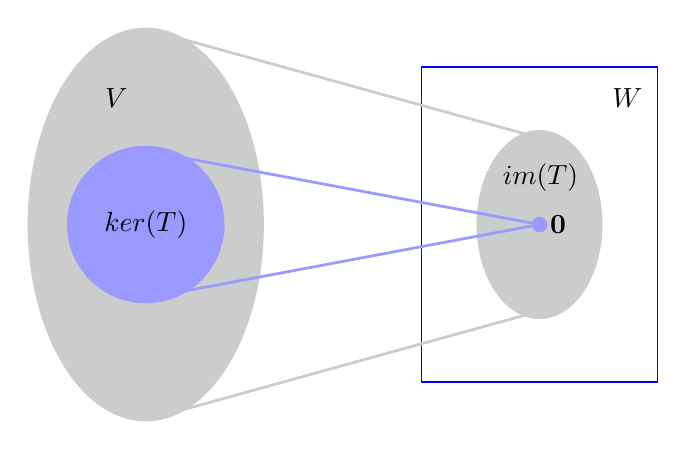
\begin{tikzpicture}
\fill[gray!40] (0,0) ellipse (1.5cm and 2.5cm);
\fill[blue!40!white] (0,0) ellipse (1cm and 1cm)node[black]{$\text{ker}(T)$};

\draw[blue] (3.5,2)node[below=4mm, right=23mm][black]{$W$} rectangle (6.5,-2);
\fill[gray!40] (5,0) ellipse (0.8cm and 1.2cm);
\fill[blue!40!white] (5,0) circle (0.1cm);

\draw[gray!40,line width=1pt](0.3,2.4)node[below=8mm, left=4mm][black]{$V$}--(5,1.1)node[below=5mm, right=-6mm][black]{$\text{im}(T)$};
\draw[gray!40, line width=1pt](0.3,-2.4)--(5,-1.1);

\draw[blue!40!white, line width=1pt](0.2,.9)--(5,0);
\draw[blue!40!white, line width=1pt](0.2,-0.9)--(5,0)node[below=0mm, right=0mm][black]{$\vec{0}$};

\end{tikzpicture}
\end{center}


\begin{example}\label{ex:kernel} Let $T:\RR^5\rightarrow \RR^4$ be a linear transformation with standard matrix $$A=\begin{bmatrix}1 & 2 & 2 &-1 & 0\\-1 & 3 & 1 & 0 & -1\\3 & 0 & 0 & 3 & 6\\ 1 & -1 & 1 & -2 & -1\end{bmatrix}$$
\begin{enumerate}
\item \label{item:kernelT}
Find $\text{ker}(T)$
\item \label{item:dimkernelT}
Is $\text{ker}(T)$ a subspace of $\RR^5$?  If so, find $\text{dim}(\text{ker}(T))$.
\end{enumerate}
\begin{explanation}
\ref{item:kernelT} To find the kernel of $T$, we need to find all vectors of $\RR^5$ that map to $\vec{0}$ in $\RR^4$.  This amounts to solving the equation $A\vec{x}=\vec{0}$.

Gauss-Jordan elimination yields:

$$\begin{bmatrix}1 & 2 & 2 &-1 & 0\\-1 & 3 & 1 & 0 & -1\\3 & 0 & 0 & 3 & 6\\ 1 & -1 & 1 & -2 & -1\end{bmatrix}  \rightsquigarrow \begin{bmatrix} 1 & 0 & 0 & 1 & 2\\0 & 1 & 0 & 1 & 1\\0 & 0 & 1 & -2 & -2\\ 0 & 0 & 0 & 0 & 0 \end{bmatrix}$$

Thus, the kernel of $T$ consists of all elements of the form:
$$\begin{bmatrix}-1\\-1\\2\\1\\0\end{bmatrix}s+\begin{bmatrix}-2\\-1\\2\\0\\1\end{bmatrix}t$$

We conclude that 
$$\text{ker}(T)=\text{span}\left(\begin{bmatrix}-1\\-1\\2\\1\\0\end{bmatrix}, \begin{bmatrix}-2\\-1\\2\\0\\1\end{bmatrix}\right)$$

\ref{item:dimkernelT}  Since $\text{ker}(T)$ is the span of two vectors of $\RR^5$, we know that $\text{ker}(T)$ is a subspace of $\RR^5$ {\color{red} reference}.  Observe that the two vectors in the spanning set are linearly independent. (How can we see this without performing computations?)  Therefore $\text{dim}(\text{ker}(T))=2$.
\end{explanation}
\end{example}

\begin{general}
Recall that the \dfn{null} of a matrix $A$ is defined to be set of all solutions to the homogeneous equation $A\vec{x}=\vec{0}$. This means that  if $T:\RR^n\rightarrow \RR^m$ is a linear transformation with standard matrix $A$ then
$$\text{ker}(T)=\text{null}(A)$$
\end{general}
We know that $\text{null}(A)$ of an $m\times n$ matrix is a subspace of $\RR^n$ {\color{red} insert reference}.  We conclude this section by showing that, in general, the kernel of a linear transformation is a subspace of the domain of the transformation.
\begin{theorem}\label{th:kersubspace} Let $T:V\rightarrow W$ be a linear transformation, then $\text{ker}(T)$ is a subspace of $V$.
\end{theorem}
\begin{proof}
To show that $\text{ker}(T)$ is a subspace, we need to show that $\text{ker}(T)$ is closed under addition and scalar multiplication.

Suppose that $\vec{v}_1$ and $\vec{v}_2$ are in $\text{ker}(T)$.  Then,
$$T(\vec{v}_1+\vec{v}_2)=T(\vec{v}_1)+T(\vec{v}_2)=\vec{0}+\vec{0}=\vec{0}$$
This shows that $\vec{v}_1+\vec{v}_2$ is in $\text{ker}(T)$.

For any scalar $a$ we have:
$$T(a\vec{v}_1)=aT(\vec{v}_1)=a\vec{0}=\vec{0}$$
This shows that $a\vec{v}_1$ is in $\text{ker}(T)$.

% {\color{red} Depending on the "subspaces of $R^n$" module, we may need to check for 0 as well}
\end{proof}

We can now define the kernel of a linear transformation.

\begin{definition}\label{def:nullityT}
The nullity of a linear transformation $T:V\rightarrow W$, is the dimension of the kernel of $T$.
$$\text{nullity}(T)=\text{dim}(\text{ker}(T))$$
\end{definition}

Notice that since the nullity of a matrix $A$ was defined as $\text{nullity}(A) = \text{dim}(\text{null}(A))$ {\color{red} need reference}, and the kernel of a linear transformation $T:\RR^n\rightarrow \RR^m$ is the null space of its associated standard matrix, our definitions of nullity are in agreement.

\section*{Rank-Nullity Theorem for Linear Transformations}

In Examples \ref{ex:image2} and \ref{ex:kernel}, we found the image and the kernel of the linear transformation $T:\RR^5\rightarrow \RR^4$ with standard matrix

$$A=\begin{bmatrix}1 & 2 & 2 &-1 & 0\\-1 & 3 & 1 & 0 & -1\\3 & 0 & 0 & 3 & 6\\ 1 & -1 & 1 & -2 & -1\end{bmatrix}$$

We also found that
$$\text{rank}(T)=\text{dim}(\text{im}(T))=\text{dim}(\text{col}(A))=\text{rank}(A)=3$$
and
$$\text{nullity}(T)=\text{dim}(\text{ker}(T))=\text{dim}(\text{null}(A))=\text{nullity}(A)=2$$

Because of Rank-Nullity Theorem {\color{red} insert reference} for matrices, it is not surprising that 
$$\text{rank}(T)+\text{nullity}(T)=3+2=5=\text{dim}(\RR^5)$$


The following theorem is a generalization of this result.

\begin{theorem}
Let $T:V\rightarrow W$ be a linear transformation.  Suppose $\text{dim}(V)=n$, then
$$\text{rank}(T)+\text{nullity}(T)=n$$
\end{theorem}

\begin{proof}
By Theorem \ref{th:imagesubspace}, $\text{im}(T)$ is a subspace of $W$.  There exists a basis for $\text{im}(T)$ of the form $\{T(\vec{v}_1), \ldots,T(\vec{v}_r)\}$.  By Theorem \ref{th:kersubspace}, $\text{ker}(T)$ is a subspace of $V$.  Let $\{\vec{u}_1,\ldots,\vec{u}_s\}$ be a basis for $\text{ker}(T)$. 

We will show that $\{\vec{u}_1,\ldots ,\vec{u}_s, \vec{v}_1,\ldots ,\vec{v}_r\}$ is a basis for $V$.

For any vector $\vec{v}$ in $V$, we have:
$$T(\vec{v})=c_1T(\vec{v}_1)+\ldots +c_rT(\vec{v}_r)$$
for some scalars $c_i$ $(1\leq i\leq r)$.
Thus, 
$$T(\vec{v})-\big(c_1T(\vec{v}_1)+\ldots +c_rT(\vec{v}_r)\big)=\vec{0}$$
By linearity,
$$T((\vec{v}-(c_1\vec{v}_1+\ldots +c_r\vec{v}_r))=\vec{0}$$
Therefore $\vec{v}-(c_1\vec{v}_1+\ldots +c_r\vec{v}_r)$ is in $\text{ker}(T)$.

Hence there are scalars $a_i$ $(1\leq i\leq s)$ such that
$$\vec{v}-(c_1\vec{v}_1+\ldots +c_r\vec{v}_r)=a_1\vec{u}_1+\ldots +a_s\vec{u}_s$$
Thus,
$$\vec{v}=(c_1\vec{v}_1+\ldots +c_r\vec{v}_r)+(a_1\vec{u}_1+\ldots +a_s\vec{u}_s)$$

We conclude that 
$$V=\text{span}(\vec{u}_1,\ldots ,\vec{u}_s, \vec{v}_1,\ldots ,\vec{v}_r)$$

Now we need to show that $\{\vec{u}_1,\ldots ,\vec{u}_s, \vec{v}_1,\ldots ,\vec{v}_r\}$ is linearly independent.

Suppose 
\begin{align}\label{eq:kerplusimproof} c_1\vec{v}_1+\ldots +c_r\vec{v}_r+a_1\vec{u}_1+\ldots +a_s\vec{u}_s=\vec{0}\end{align}
Applying $T$ to both sides, we get
$$T(c_1\vec{v}_1+\ldots +c_r\vec{v}_r+a_1\vec{u}_1+\ldots +a_s\vec{u}_s)=T(\vec{0})$$
$$c_1T(\vec{v}_1)+\ldots +c_rT(\vec{v}_r)+a_1T(\vec{u}_1)+\ldots +a_sT(\vec{u}_s)=\vec{0}$$

But $T(\vec{u}_i)=\vec{0}$ for $1\leq i\leq s$, thus
$$c_1T(\vec{v}_1)+\ldots +c_rT(\vec{v}_r)=\vec{0}$$
Since $\{T(\vec{v}_1),\ldots ,T(\vec{v}_r)\}$ is linearly independent, it follows that each $c_i=0$.  

But then Equation (\ref{eq:kerplusimproof}) implies that $a_1\vec{u}_1+\ldots +a_s\vec{u}_s=\vec{0}$.  Because $\{\vec{u}_1, \ldots ,\vec{u}_s\}$ is linearly independent, it follows that each $a_i=0$.  

We conclude that $\{\vec{u}_1,\ldots ,\vec{u}_s,\vec{v}_1,\ldots ,\vec{v}_r\}$ is a basis for $V$.  Thus,

$$\text{dim}(\text{ker}(T))+\text{dim}(\text{im}(T))=s+r=n$$
\end{proof}

\section*{Practice Problems}
\begin{problem}
Describe the image and find the rank for each linear transformation $T:\RR^n\rightarrow \RR^m$ with standard matrix $A$ given below.
  \begin{problem}
  $T:\RR^5\rightarrow \RR^2$, $A=\begin{bmatrix}3&2&4&7&1\\-1&-9&7&6&8\end{bmatrix}$.
  
  \begin{multipleChoice}
  \choice[correct]{$\text{im}(T)=\RR^2$}
  \choice{$\text{im}(T)$ is a line in $\RR^2$}
  \choice{$\text{im}(T)=\{\vec{0}\}$ }
  \choice{$\text{im}(T)=\RR^5$}
  \choice{$\text{im}(T)$ is a plane in $\RR^5$}
\end{multipleChoice}
  
  $\text{rank}(T)=\answer{2}$
  \end{problem}
  
  \begin{problem}
  $T:\RR^2\rightarrow\RR^3$, $A=\begin{bmatrix}1&1\\1&1\\1&1\end{bmatrix}$
  
  \begin{multipleChoice}
  \choice{$\text{im}(T)=\RR^3$}
  \choice{$\text{im}(T)$ is a line in $\RR^2$}
  \choice[correct]{$\text{im}(T)$ is a line in $\RR^3$}
  \choice{$\text{im}(T)=\{\vec{0}\}$ }
  \choice{$\text{im}(T)$ is a plane in $\RR^3$}
\end{multipleChoice}
  
  $\text{rank}(T)=\answer{1}$
  \end{problem}
\end{problem}


\begin{problem} Suppose linear transformations $T:\RR^2\rightarrow \RR^2$ and $S:\RR^2\rightarrow \RR^2$ are such that  $\text{im}(T)=\text{im}(S)=\text{span}\left(\begin{bmatrix}1\\-3\end{bmatrix}\right)$.  Does this mean that $T$ and $S$ are the same transformation?  Justify your claim.
\end{problem}

\begin{problem}
Describe the kernel and find the nullity for each linear transformation $T:\RR^n\rightarrow \RR^m$ with standard matrix $A$ given below.

\begin{problem}
$T:\RR^3\rightarrow \RR^2$, $A=\begin{bmatrix}2&1&0\\-1&1&-3\end{bmatrix}$.

\begin{multipleChoice}
  \choice{$\text{ker}(T)=\RR^3$}
  \choice{$\text{ker}(T)=\{\vec{0}\}$ }
  \choice{$\text{ker}(T)=\RR^2$}
  \choice{$\text{ker}(T)$ is a plane in $\RR^3$}
   \choice[correct]{$\text{ker}(T)$ is a line in $\RR^3$}
\end{multipleChoice}

$\text{nullity}(T)=\answer{1}$
\end{problem}

\begin{problem}
$T:\RR^2\rightarrow \RR^2$, $A=\begin{bmatrix}2&-1\\3&0\end{bmatrix}$.

\begin{multipleChoice}
  \choice{$\text{ker}(T)=\RR^2$}
  \choice[correct]{$\text{ker}(T)=\{\vec{0}\}$ }
   \choice{$\text{ker}(T)$ is a line in $\RR^2$}
\end{multipleChoice}

$\text{nullity}(T)=\answer{0}$
\end{problem}

\begin{problem}
$T:\RR^3\rightarrow \RR^5$, $A=\begin{bmatrix}1&2&-1\\1&2&-1\\1&2&-1\\1&2&-1\\1&2&-1\end{bmatrix}$ 

\begin{multipleChoice}
 \choice[correct]{$\text{ker}(T)$ is a plane in $\RR^3$}
 \choice{$\text{ker}(T)$ is a line in $\RR^3$}
     \choice{$\text{ker}(T)$ is a line in $\RR^5$}
 \choice{$\text{ker}(T)=\RR^3$}
  \choice{$\text{ker}(T)=\{\vec{0}\}$ }
  
\end{multipleChoice}

$\text{nullity}(T)=\answer{2}$
\end{problem}
\end{problem}

\begin{problem}
Suppose a linear transformation $T:\RR^3\rightarrow \RR^3$ is such that $\text{im}(T)$ is a plane in $\RR^3$.  Then
$$\text{rank}(T)=\answer{2}$$ $$\text{nullity}(T)=\answer{1}$$
\end{problem}

\begin{problem}
Suppose a linear transformation $T:\RR^5\rightarrow \RR^5$ is such that $T(\vec{v})=\vec{0}$ for all $\vec{v}$ in $\RR^5$.  Then
$$\text{rank}(T)=\answer{0}$$ $$\text{nullity}(T)=\answer{5}$$
\end{problem}

\begin{problem} Let $T:\RR^6\rightarrow \RR^4$ be a linear transformation with standard matrix
$$A=\begin{bmatrix}2&-1&1&-2&1&1\\1&2&3&6&-4&1\\0&2&2&4&-2&-1\\1&3&2&6&-3&2\end{bmatrix}$$
Find $\text{im}(T)$ and $\text{ker}(T)$ if the reduced row-echelon form of $A$ is 
$$\text{rref}(A)=\begin{bmatrix}1&0&0&1&-1&0\\0&1&0&1&0&0\\0&0&1&1&-1&0\\0&0&0&0&0&1\end{bmatrix}$$
\end{problem}
\begin{problem} Let $V=\text{span}\left(\begin{bmatrix}1\\1\end{bmatrix}\right)$, and let $T:V\rightarrow \RR^2$ be a linear transformation defined by 
$T(\vec{v})=2\vec{v}$.  Find $\text{im}(T)$ and $\text{ker}(T)$.
\end{problem}

\begin{problem}
Suppose a linear transformation $T$ is induced by a $4\times 6$ matrix $A$.  Let $S$ be a linear transformation induced by $A^T$.  Find $\text{nullity}(S)$, if $\text{nullity}(T)=3$.  Prove your claim.
\end{problem}




\end{document}
